\documentclass[11pt,a4paper]{ctexart}
\usepackage{fontspec}
\defaultfontfeatures{Mapping=tex-text}
\usepackage{xunicode}
\usepackage{xltxtra}
%\setmainfont{???}
\usepackage{amsmath}
\usepackage{amsfonts}
\usepackage{amssymb}
\usepackage{graphicx}
\usepackage{amsthm}
\usepackage{array}
\usepackage{float}   %{H}
\usepackage{booktabs}  %\toprule[1.5pt]
\usepackage[titletoc]{appendix}
%===================%插入代码需要的控制
\usepackage{listings}
\usepackage{xcolor}
\setmonofont{Consolas}%字体
\lstset{
	numbers=left, 
	numberstyle= \tiny, 
	keywordstyle= \color{ blue!70},
	commentstyle= \color{red!50!green!50!blue!50}, 
	frame=shadowbox, % 阴影效果
	rulesepcolor= \color{ red!20!green!20!blue!20} ,
	escapeinside=``,% 英文分号中可写入中文
	basicstyle=\ttfamily 
} 
%===================%
\usepackage[left=2cm,right=2cm,top=2cm,bottom=2cm]{geometry}

\newtheorem{theorem}{定理}
\newtheorem{definition}{定义}
\newtheorem*{solution}{解}
\newtheorem{practice}{题}

\title{多元统计分析(2)}
\author{钟瑜 \quad 222018314210044}
\date{\today}
\begin{document}
	\maketitle
	\pagestyle{plain}%设置页码
\begin{figure}[H]
	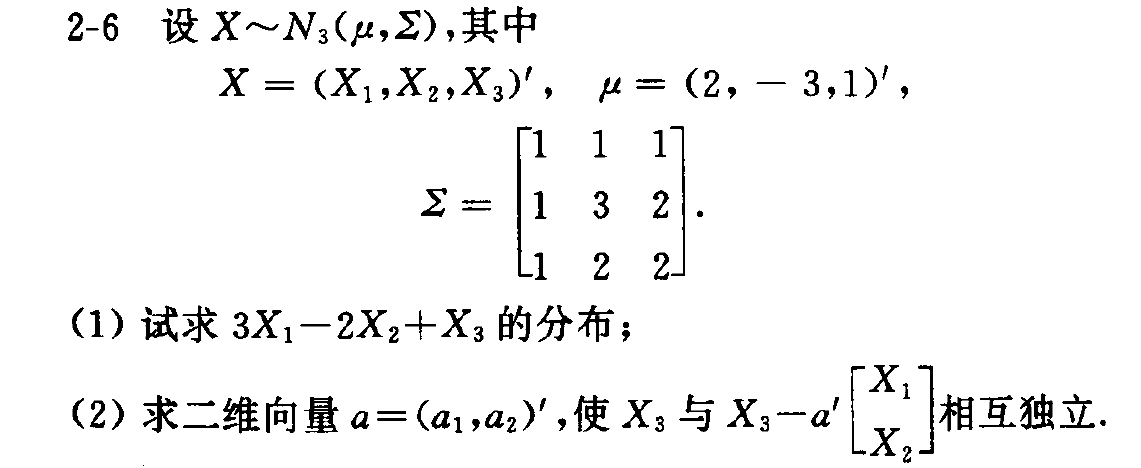
\includegraphics[width=0.7\textwidth]{1.png}
\end{figure}
\begin{solution}
	\begin{enumerate}
		\item [(1)]由于$ 3X_1-2X_2+X_3=(3,-2,1)X=a'X $,故$ 3X_1-2X_2+X_3 $服从$ N(a'\mu,a'\Sigma a) =N(25,9)$,其中
		\begin{equation}
		a'\mu=(3,-2,1)\mu=13
		\end{equation}
	\[
	a'\Sigma a=(3,-2,1) \left(
	\begin{array}{ccc}
		1& 1 & 1\\
		1& 3 & 2\\
		1& 2 & 2\\
	\end{array} \right)(3,-2,1)'=9
	\]
		\item [(2)] 由于$ X_3\sim N(1,2) $, 而$$ X_3-a'(X_1,X_2)' =X_3-a_1X_1-a_2X_2=(-a_1,-a_2,1)X=b'X\sim N(b'\mu, b'\Sigma b)$$
		要使得$ X_3 $与$ b'X $独立,则$ cov(X_3,b'X)=0 $
		\begin{equation}
			\begin{aligned}
			cov(X_3,b'X) &= \mathbb{E}[(X_3-\mu_3)(b'X-b'\mu)]\\
			&=  \mathbb{E}[X_3b'X]-2b'\mu\\
			&= \mathbb{E}[X_3(-a_1,-a_2,1)X]-2b'\mu\\
			&= 0
			\end{aligned}
		\end{equation}
	即
	$$ \mathbb{E}[-a_1X_3X_1-a_2X_2X_3+X_3X_3]=-6a_1+9a_2+3 $$
	而
	$$\mathbb{E}[X_3X_1]=cov(X_3,X_1)+\mathbb{E}X_1\mathbb{E}X_3=3$$
	$$\mathbb{E}[X_3X_2]=cov(X_3,X_2)+\mathbb{E}X_2\mathbb{E}X_3=-1$$
	$$\mathbb{E}[X_3X_3]=var(X_3)+\mathbb{E}X_3^2=1$$
	代入得$ a_1+a_2-2=0 $.
	\end{enumerate}
\end{solution}
\begin{figure}[H]
	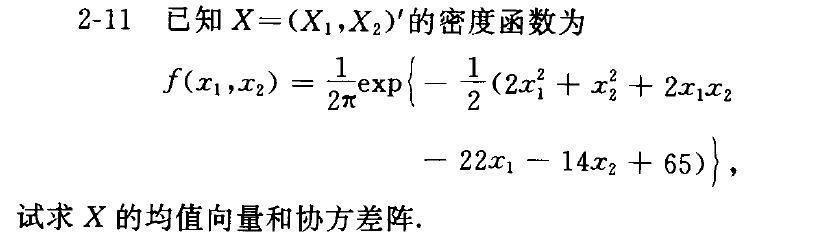
\includegraphics[width=0.7\textwidth]{2.png}
\end{figure}
\begin{solution}
首先求出$ X_1 $和$ X_2 $的边缘分布:

\begin{equation}
\begin{aligned}
f_{X_1}(x) &= \int_{-\infty}^{\infty}f(x_1,x_2)dx_2\\
&= \frac{1}{2\pi}\int_{-\infty}^{\infty}exp\left\lbrace -\frac{1}{2}(2x_1^2+x_2^2+2x_1x_2-22x_1-14x_2+65)\right\rbrace dx_2\\
&= \frac{1}{2\pi}exp\left\lbrace -\frac{1}{2}(2x_1^2-22x_1+65)\right\rbrace \int_{-\infty}^{\infty}exp\left\lbrace -\frac{1}{2}(x_2^2+2x_1x_2-14x_2)\right\rbrace dx_2\\
&= \frac{1}{2\pi}exp\left\lbrace -\frac{1}{2}(2x_1^2-22x_1+65)\right\rbrace \int_{-\infty}^{\infty}exp\left\lbrace -\frac{1}{2}(x_2^2+2x_2(x_1-7)+(x_1-7)^2)\right\rbrace d exp\left\lbrace -\frac{1}{2}(x_1-7)^2\right\rbrace x_2 \\
&=  \frac{1}{2\pi}exp\left\lbrace -\frac{1}{2}(2x_1^2-22x_1+65)\right\rbrace exp\left\lbrace -\frac{1}{2}(x_1-7)^2 \right\rbrace \int_{-\infty}^{\infty}exp\left\lbrace -\frac{1}{2}(x_2^2+2x_2(x_1-7)+(x_1-7)^2)\right\rbrace  dx_2 \\
&= \frac{1}{\sqrt{2\pi}}exp\left\lbrace -\frac{1}{2}(x_1^2-8x_1+16)\right\rbrace \frac{1}{\sqrt{2\pi}}
\int_{-\infty}^{\infty}exp\left\lbrace -\frac{1}{2}(x_2-x_1+7)^2\right\rbrace  dx_2 \\
&= \frac{1}{\sqrt{2\pi}}exp\left\lbrace -\frac{1}{2}(x_1-4)^2\right\rbrace 
\end{aligned}
\end{equation}
因此$ X_1\sim N(4,1) $
同理可得$ X_2\sim N(3,2) $
故均值向量$ \mu=(4,3)' $.

然后计算$ X_1 $和$ X_2 $的协方差.
\begin{equation}
\begin{aligned}
cov(X_1,X_2) &=\mathbb{E}[(X_1-4)(X_2-3)]\\
&= \iint^{\infty}_{-\infty}(x_1-4)(x_2-3)f(x_1,x_2)dx_1dx_2\\
&= \iint^{\infty}_{-\infty}a_1a_2\frac{1}{2\pi}exp\left\lbrace -\frac{1}{2}(2a_1^2+a_2^2+2a_1a_2)\right\rbrace da_1da_2(\mbox{其中}a_1=x_1-4,a_2=x_2-3)\\
&= \frac{1}{\sqrt{2\pi}}\int_{-\infty}^{\infty}a_1exp\left\lbrace -\frac{a_1^2}{2}\right\rbrace \left[ \int_{-\infty}^{\infty}\frac{1}{\sqrt{2\pi}}a_2exp\left\lbrace -\frac{1}{2}(a_1+a_2)^2\right\rbrace da_2 \right] da_1\\
&= \frac{1}{\sqrt{2\pi}}\int_{-\infty}^{\infty}a_1exp\left\lbrace -\frac{a_1^2}{2}\right\rbrace \frac{1}{\sqrt{2\pi}}\left[ \int_{-\infty}^{\infty}(a_1+a_2-a_1)exp\left\lbrace -\frac{1}{2}(a_1+a_2)^2\right\rbrace da_2 \right]da_1\\
&=-1
\end{aligned}
\end{equation}
因此协方差矩阵为:
\[
\Sigma= \left(
\begin{array}{cc}
	 1 & -1\\
	 -1 & 2\\
\end{array} \right)
\]
\end{solution}
\begin{figure}[H]
	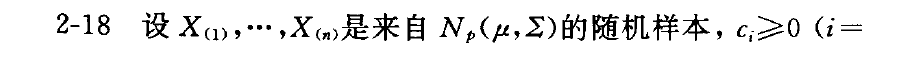
\includegraphics[width=0.7\textwidth]{3.png}
\end{figure}
\begin{figure}[H]
	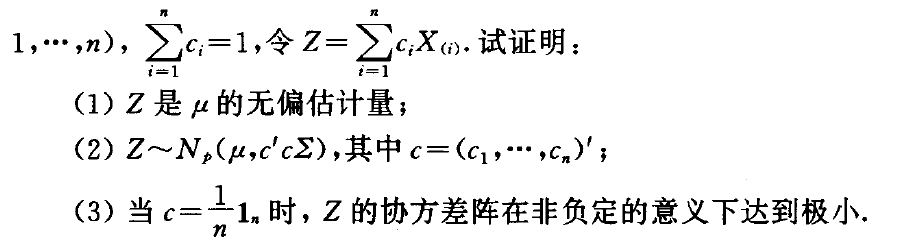
\includegraphics[width=0.7\textwidth]{4.png}
\end{figure}
\begin{solution}
\begin{enumerate}
	\item [(1)] 
	$ \mathbb{E}Z= \mathbb{E}(\sum_{i=1}^{n}c_iX_{(i)})=\sum_{i=1}^{n}c_i\mathbb{E}X_{(i)}=\sum_{i=1}^{n}c_i\mu=\mu$
	\item [(2)] 因为$ X_{(i)}\sim N_p(\mu,\Sigma) $,故对每个i,$ X_{(i)} $的特征函数为:
	\begin{equation}
	\phi(t)=\mathbb{E}(e^{itX_{(i)}})=exp\left[ it'\mu-\frac{1}{2}t'\Sigma t\right] 
	\end{equation}
	由于Z=$\sum_{i=1}^{n}c_iX(i) $,故Z的特征函数为:
	\begin{equation}
	\begin{aligned}
	\phi_Z(t) &=\mathbb{E}(e^{itZ})\\
	&= \mathbb{E}(e^{it\sum_{i=1}^{n}c_iX_{(i)}})\\
	&= \prod_{i=1}^{n}\mathbb{E}(e^{ic_itX_{(i)}})\\
	&= \prod_{i=1}^{n}exp\left[ ic_it'\mu-\frac{1}{2}(c_it)'\Sigma (c_it)\right] \\
	&= \prod_{i=1}^{n}exp\left[ ic_it'\mu-\frac{1}{2}c_i^2t'\Sigma t\right] \\
	&= exp\left[ i\sum_{i=1}^{n}c_it'\mu-\frac{1}{2}\sum_{i=1}^{n}c_i^2t'\Sigma t\right] \\
	&= exp\left[ it'\mu-\frac{1}{2}t'(c_i'c_i\Sigma )t\right] \\
	\end{aligned}
	\end{equation}
因此$ Z\sim N_p(\mu,c_i'c_i\Sigma) $.
	\item [(3)] 由均值不等式,
		\begin{equation}
		\begin{aligned}
		c'c &= \sum_{i=1}^{n}c_i^2
		&\geq (\sum_{i=1}^{n}c_i)^2/n
		\end{aligned}
    	\end{equation}
	当且仅当$ c_1=...=c_n $时,即$ c=\frac{1}{n}\textbf{1}_n $,Z的协方差阵在非负定意义下达到极小,为$ c_i'c_i\Sigma = \frac{1}{n}\Sigma $
\end{enumerate}
\end{solution}
\begin{figure}[H]
	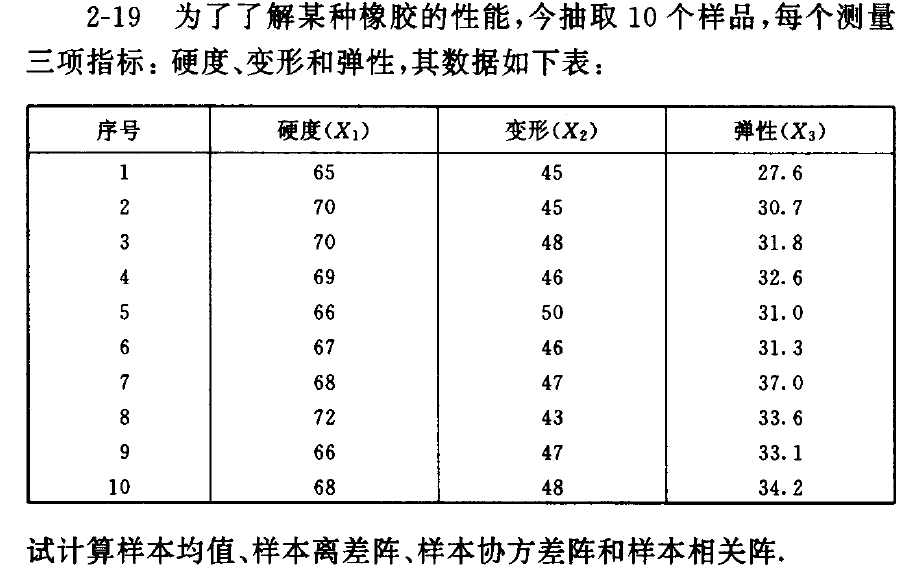
\includegraphics[width=0.7\textwidth]{5.png}
\end{figure}
\begin{solution}
R运算结果如下:
\end{solution}
\begin{lstlisting}[language=r]
> rubber<-read.csv("E:/4.多元统计分析/zuoye/2/1.csv")
> rubber
   num X1 X2   X3
1    1 65 45 27.6
2    2 70 45 30.7
3    3 70 48 31.8
4    4 69 46 32.6
5    5 66 50 31.0
6    6 67 46 31.3
7    7 68 47 37.0
8    8 72 43 33.6
9    9 66 47 33.1
10  10 68 48 34.2

> mean(rubber$X1)   #样本均值
[1] 68.1
> mean(rubber$X2)
[1] 46.5
> mean(rubber$X3)
[1] 32.29

> cov(rubber[-1])   #样本协方差阵
          X1         X2        X3
X1  4.766667 -1.9444444 1.9344444
X2 -1.944444  3.8333333 0.6166667
X3  1.934444  0.6166667 6.1898889

> 9*cov(rubber[-1])    #样本离差阵
       X1     X2     X3
X1  42.90 -17.50 17.410
X2 -17.50  34.50  5.550
X3  17.41   5.55 55.709

> cor(rubber[-1])   #样本相关阵
           X1         X2        X3
X1  1.0000000 -0.4548832 0.3561291
X2 -0.4548832  1.0000000 0.1265962
X3  0.3561291  0.1265962 1.0000000

\end{lstlisting}

\end{document}